\documentclass[border=3pt]{standalone}
% Preâmbulo compartilhado pelos diagramas TikZ da aula 10 (Localização de Markov e Gaussiana)
\usepackage[T1]{fontenc}
\usepackage[utf8]{inputenc}
\usepackage{lmodern}
\usepackage{amsmath}
\usepackage{xcolor}
\usepackage{tikz}
\usetikzlibrary{arrows.meta,angles,quotes,decorations.pathmorphing,calc,
                positioning,shapes.geometric,shapes.misc,backgrounds,fit,
                math}

% Paleta (mesma dos SVGs originais)
\definecolor{dblue}{HTML}{2A5B8C}
\definecolor{dorange}{HTML}{B3541E}
\definecolor{dgreen}{HTML}{4A7C59}
\definecolor{dred}{HTML}{9C4B4B}
\definecolor{dcream}{HTML}{F4F1EA}
\definecolor{dshade}{HTML}{DDD7C9}

% Função gaussiana (não normalizada por padrão de escala visual)
\pgfmathdeclarefunction{gauss}{3}{%
  \pgfmathparse{1/(#3*sqrt(2*pi))*exp(-((#1-#2)^2)/(2*#3^2))}%
}

% Estilos comuns (prefixo d... para não colidir com chaves internas do pgf)
\tikzset{
  >={Stealth[length=2mm]},
  dguide/.style={gray!55, dashed, line width=0.4pt},
  daxis/.style={gray!60, line width=0.7pt, ->},
  dbody/.style={fill=black!3, draw=black!80, line width=1pt},
  dacc/.style={draw=dblue, line width=1pt},
  dlbl/.style={black!55, font=\small},
  dsub/.style={black!45, font=\footnotesize},
  dstate/.style={circle, draw=black!80, fill=dcream, line width=1pt,
                 minimum size=17mm, font=\large, inner sep=1pt},
  dobs/.style={circle, draw=black!80, fill=dshade, line width=1pt,
               minimum size=14mm, font=\large, inner sep=1pt},
  dbox/.style={rounded corners=2pt, draw=black!80, fill=dcream, line width=1pt,
               align=center, inner sep=6pt},
  dop/.style={circle, draw=black!80, fill=white, line width=1pt,
              minimum size=6mm, inner sep=0pt, font=\small},
  dtrans/.style={->, dblue, line width=1pt},
  dmeas/.style={->, dorange, line width=1pt},
  dcurve/.style={line width=1pt, dblue},
  dcurveb/.style={line width=1.4pt, dorange},
}

\usetikzlibrary{shapes.callouts}
\begin{document}
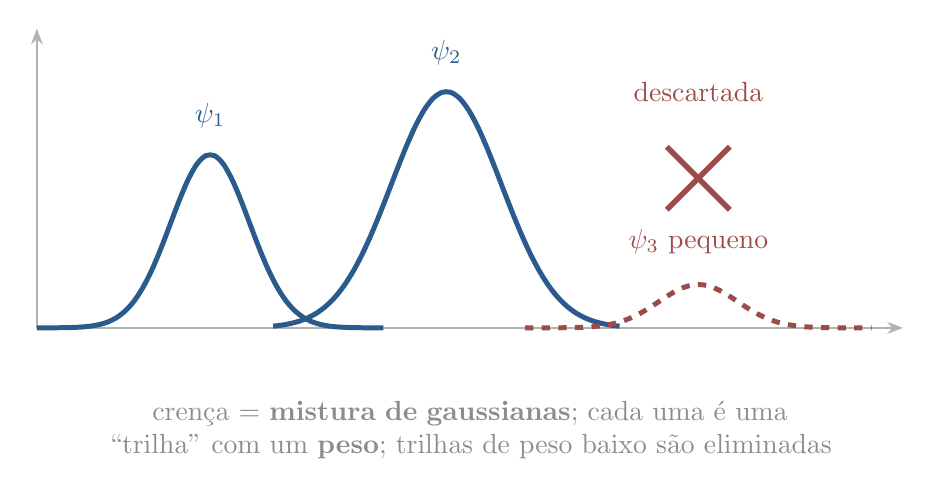
\begin{tikzpicture}[x=1cm,y=1cm,bal/.style={rectangle callout, rounded corners=7pt, draw=black!75, fill=white, line width=1pt, align=center, font=\normalsize, inner sep=5pt}]
\draw[daxis] (0,0) -- (11,0); \draw[daxis] (0,0) -- (0,3.8);
\draw[dblue, line width=1.8pt, domain=0.0:4.4, samples=40, smooth] plot (\x,{2.20*exp(-((\x-2.20)*(\x-2.20))/(2*0.50*0.50))});
\draw[dblue, line width=1.8pt, domain=3.0:7.4, samples=40, smooth] plot (\x,{3.00*exp(-((\x-5.20)*(\x-5.20))/(2*0.70*0.70))});
\draw[dred, line width=1.8pt, dashed, domain=6.2:10.6, samples=40, smooth] plot (\x,{0.55*exp(-((\x-8.40)*(\x-8.40))/(2*0.50*0.50))});
\node[dblue, font=\normalsize] at (2.2,2.7) {$\psi_1$}; \node[dblue, font=\normalsize] at (5.2,3.5) {$\psi_2$}; \node[dred, font=\normalsize] at (8.4,1.1) {$\psi_3$ pequeno};
\draw[dred, line width=2pt] (8.0,1.5) -- (8.8,2.3) (8.0,2.3) -- (8.8,1.5); \node[dred, font=\normalsize, align=center] at (8.4,3.0) {descartada};
\node[dsub, font=\normalsize, align=center, text width=11cm] at (5.5,-1.3) {crença = \textbf{mistura de gaussianas}; cada uma é uma ``trilha'' com um \textbf{peso}; trilhas de peso baixo são eliminadas};
\end{tikzpicture}
\end{document}
